\documentclass[tikz,border=12pt]{standalone}
% Estilo comum dos esquemas vetoriais das aulas da GA033.
\usepackage[T1]{fontenc}
\usepackage[utf8]{inputenc}
\usepackage{lmodern}
\usepackage{amsmath,amssymb}
\usetikzlibrary{arrows.meta,positioning,calc,fit,matrix,decorations.pathreplacing,backgrounds,shapes.geometric}
\definecolor{lnccblue}{HTML}{075AC0}
\definecolor{ink}{HTML}{242A31}
\definecolor{muted}{HTML}{647080}
\definecolor{lightblue}{HTML}{EFF5FC}
\definecolor{teal}{HTML}{197C83}
\definecolor{orange}{HTML}{BC6A16}
\tikzset{
  every node/.style={font=\sffamily\fontsize{15}{18}\selectfont,text=ink},
  box/.style={draw=lnccblue,line width=0.9pt,fill=lightblue,inner sep=9pt,align=center},
  flow/.style={-{Stealth[length=3mm,width=2mm]},draw=lnccblue,line width=1pt},
  point/.style={circle,draw=lnccblue,fill=white,line width=1.2pt,minimum size=3.2mm,inner sep=0pt},
  label/.style={font=\sffamily\fontsize{13}{16}\selectfont,text=muted},
  heading/.style={font=\sffamily\bfseries\fontsize{16}{19}\selectfont,text=lnccblue}
}
% Impede setas horizontais involuntariamente invertidas após editar os nós.
\newdimen\origemseta
\newdimen\destinoseta
\newcommand{\verificarsetadireita}[2]{%
  \pgfextractx{\origemseta}{\pgfpointanchor{#1}{east}}%
  \pgfextractx{\destinoseta}{\pgfpointanchor{#2}{west}}%
  \advance\origemseta by 4mm%
  \ifdim\destinoseta>\origemseta\else
    \PackageError{diagramas}{Conector sem espaco entre #1 e #2}{Afaste os nos antes de compilar.}%
  \fi
}

\begin{document}
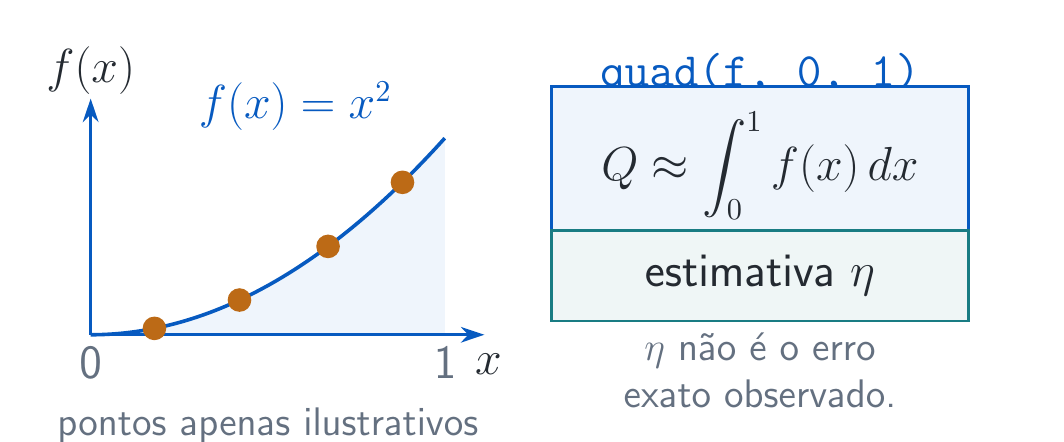
\begin{tikzpicture}[x=1cm,y=1cm,
  every node/.append style={font=\sffamily\fontsize{16}{19}\selectfont}]
  \path[use as bounding box] (0,0) rectangle (12.8,4.9);
  \fill[lightblue] (.8,1.0) -- plot[domain=0:1,samples=80]
    ({.8+4.5*\x},{1.0+2.5*\x*\x}) -- (5.3,1.0) -- cycle;
  \draw[flow] (.8,1.0) -- (5.8,1.0);
  \draw[flow] (.8,1.0) -- (.8,4.0);
  \draw[lnccblue,line width=1.3pt] plot[domain=0:1,samples=80]
    ({.8+4.5*\x},{1.0+2.5*\x*\x});
  \foreach \t in {.18,.42,.67,.88} {
    \fill[orange] ({.8+4.5*\t},{1.0+2.5*\t*\t}) circle[radius=1.5mm];
  }
  \node at (5.85,.62) {$x$};
  \node at (.8,4.35) {$f(x)$};
  \node[text=muted] at (.8,.65) {0};
  \node[text=muted] at (5.3,.65) {1};
  \node[heading] at (3.4,3.9) {$f(x)=x^2$};
  \node[text=muted,font=\sffamily\fontsize{14}{17}\selectfont] at (3.05,-.15) {pontos apenas ilustrativos};
  \node[heading] at (9.3,4.3) {\texttt{quad(f, 0, 1)}};
  \node[box,minimum width=5.3cm,minimum height=.9cm] at (9.3,3.15)
    {$Q\approx\displaystyle\int_0^1 f(x)\,dx$};
  \node[box,draw=teal,fill=teal!7,minimum width=5.3cm,minimum height=.9cm] at (9.3,1.75)
    {estimativa $\eta$};
  \node[text=muted,align=center,text width=5.3cm,font=\sffamily\fontsize{14}{17}\selectfont] at (9.3,.55) {$\eta$ não é o erro\\exato observado.};
\end{tikzpicture}
\end{document}
